\chapter{Zeitplan}  % Kapitel % Steht dann über dem Text
\label{chapter:Zeitplan}  % Steht als Text im Inhaltsverzeichnis
\index{Zeitplan} % für das Stichwortverzeichnis
\begin{figure}[h]
\begin{center}
   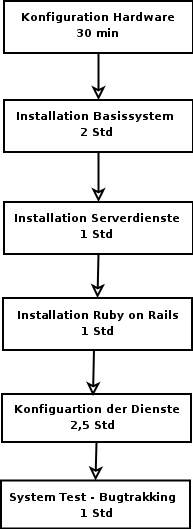
\includegraphics[width=5cm]{../bilder/Zeitplaninstall.png}
   \caption{Zeitplan Systeminstallation}
   \label{Zeitplan-Ablauf}
\end{center}
\end{figure}

Die Grafik zeigt den ideal Ablauf einer Serverinstallation für einen CodeRed Server. Probleme mit der Hardware oder auch mit der Anbindung sind hier nicht berücksichtigt. Die Intallation kann sich bei Problemen, die nichts direkt mit dem eigentlichen System zutun haben, um eine nicht bestimmbare Zeit verlängern.


